\documentclass{article}

%Language and Encoding
\usepackage[francais]{babel}
\usepackage[utf8]{inputenc}

%Images
\usepackage{graphicx} 

%Algorithm 
\usepackage{algorithmic}
\usepackage{algorithm}


%Info
\title{\textbf{Contrôle d'accès e le POSIX Access Control Lists(ACL)} \\ CS435 - Administration de Système }
\author{Dan Pham et Fabrício Nascimento}
\date{Octobre 2009}

\begin{document}

\maketitle
\newpage

%VOIR
\tableofcontents
\newpage

\section{Introduction}
%Problème et solution plus simple
Quand on désire contrôler l'accès aux données dans un système de fichiers, il y a plusieurs moyens d’y parvenir. Par défaut, les systèmes POSIX (Portable Operation System Interface)\cite{ieee1,ieee2} ont un mécanisme qui permet d’associer chaque entité avec un ensemble de règles, lequel est composé par une séquence d'octet qui exprime les droits du propriétaire, de son groupe et des autres utilisateurs.

%Les limitations de cette solution
Ce mode, traditionnel, assez simple est capable de résoudre les problèmes les plus fréquents. Par contre, il pose des limitations aux administrateurs de systèmes qui pour exprimer leurs besoins doivent employer des configurations non évidentes. Pour cette raison, certaines applications choisissent de développer leur propre système de droit, comme le serveur FTP Proftp\cite{ftp} pour résoudre ce problèmes de droits.

% La solution ACL
Pour remédier à ces limitations, les systèmes UNIX peuvent employer les ACL. Cet article présente une exposition sur les ACL POSIX, ses modes de fonctionnement, ses qualités et désavantages. Le texte s’inspire de l'article d’Andreas Gruembacher\cite{aclsuse} qui a fait partit de l’équipe ayant ajouté le support aux ACL dans le noyaux Linux pour les systèmes de fichiers ext2 et ext3, qui sont les plus utilisés dans les monde UNIX.

\section{Le POSIX 1003.1}
 
Traditionnellement les systèmes qui implémentaient la norme POSIX avaient un système simple et puissant de permissions mais qui cependant posait certains problèmes. En effet, les différentes versions d'ACL disponibles étaient incompatibles entre elles.
 
Pour normaliser les problème de sécurité sur les systèmes POSIX (ACL en faisant partie), un groupe a été formé pendant la définition de la famille de normes POSIX 1003.1. Les premiers documents POSIX qui ont pris en compte ces questions étaient les documents 1003.1e (\emph{System Application Programming Interface}) et 1003.2c (\emph{Shell and Utilities}), cependant, le premier draft était trop ambitieux. En effet, le groupe responsable pour la normalisation avait divisé ses efforts sur un grand nombre de domaines qui comportaient les \emph{Access Control Lists} (ACL), les \emph{Audit}, les \emph{Capability},les \emph{ Mandatory Access Control }(MAC), et l'\emph{Information Labeling}\cite{aclsuse}.
 
En Janvier de 1998\cite{aclsuse} le financement pour ce projet à été suspendu, par contre, le travail n'était pas prêt. De toute façon le dixsèptieme draft a quand même été rendu public\cite{posix17}.
 
Après cette publication, des systèmes UNIX appelés "\emph{trusted}" (Trusted Solaris, Trusted Irix, Trusted AIX) ont été développés à partir du draft 17. Ces systèmes ne sont pas complètement compatibles entre eux. Heureusement aujourd'hui la plupart des systèmes UNIX et UNIX-like supportent les ACL. Ces implémentations sont usuellement compatibles avec le draft 17. Le projet TrustedBSD implémente aussi les ACL sur les système BSD. Les ACL sont apparues sur les Macs en 2003 avec la RELEASE MAC FreeBSD.
 
Les ACL sont une évolution du système de permissions traditionnel présent dans pratiquement tous les systèmes UNIX, alors, avant d'expliquer les ACL on va d'abord parler du modèle traditionnel.

\section{Système de permissions traditionnel}
 
%Les groups et les permissions
Le modèle traditionnel POSIX offre trois classes d'utilisateurs qui sont: le propriétaire (\emph{owner}), le groupe propriétaire (\emph{group}) et les autres utilisateurs (\emph{others}). Chaque groupe a un octet que indique les permissions de lecture (\emph{\textbf{r}ead}), d'écriture (\emph{\textbf{w}rite}) et d'exécution (\emph{e\textbf{x}ecute}).
 
%Explication simple
Après les trois octets peut venir le \emph{Set User Id}, \emph{Set Group Id} et le \emph{Sticky Bit} qui peuvent être utilisés dans certain cas. Il faut faire attention avec le \emph{Sticky Bit}, il permet aux utilisateurs normaux d'exécuter les utilitaires comme l'administrateur(\emph{root}), donc une faille de sécurité dans une application utilisant le \emph{Sticky Bit} peut compromettre le système entier.
 
%Le droit du root
Seul le \emph{root} peut créer les groupes et changer les associations de groupes. Il peut aussi changer les propriétaires.
 
\section{Les ACL}
 
%Definitions de base
Chaque ACL est une ensemble de règles d'accès. Dans une modèle de sécurité utilisant les ACL, si une entité fait une requête pour accéder aux données, il faut consulter les la liste d'ACL pour savoir si nous avons la permission pour l'opération demandé. Les règles possibles peuvent être consultées dans le tableau ci-dessous(\ref{entree}).

\begin{center}
\begin{tabular}{|l|l|}
  \hline
    \multicolumn{2}{|c|}{Les types de ACL} \\
  \hline
\textbf{Type d'entrée} & \textbf{format} \\
  \hline
Propriétaire & user::rwx \\
Utilisateur nommée & user:name:rwx \\
Groupe propriétaire & group::rwx \\
Groupe nommée & group:name:rwx \\
Masque & mask::rwx \\
Autres & other::rwx \\
  \hline
\end{tabular}
\label{tab:entree}
\end{center}
 
Les règles sont formées par un indicateur de classe (comme les classes du système traditionnel), l'identificateur pour préciser de quel utilisateur ou groupe on parle puis les octets de permissions.

Les ACL équivalentes au mode simple de permissions s'appellent les ACL minimales. Une ACL minimale possède 3 entrée (propriétaire, groupe propriétaire et autres) qu'on peut convertir directement. Si les ACL possèdent des entrées supplémentaires, ont les appelle ACL étendues. Toutes les ACL étendues doivent avoir une entrée masque et peuvent contenir théoriquement autant d'entrées que l'on désire. Ce numéro d'entrée peut-être limitée pour chaque implémentation et qu'il est aussi important pour les performances.

Quelquefois on a des application qui ne sont pas programmer pour fonctionner avec les ACL, cela veut dire que l'on doit créer une relation pour convertir les ACL vers le système traditionnel, de façon que ces application ne donnerons pas de façon inattendue plusieurs droits aux utilisateurs ou groupes. 

Quand le programme utilise des ACL minimales ce problème n'arrive jamais: la relation entre ces ACL et le système traditionnel est directe. Par contre, dans les ACL étendues cela pose une problème. Les propriétaires et les autres seront directement associe avec les classes de même nom, par contre, les entrées de groupe et utilisateur nommé avec le groupe propriétaire seront tous associés avec la classe du groupe propriétaire. Par conséquent, le sens du classe groupe propriétaire doit être redéfinie comme la limite supérieure des permissions de chaque entrée dans pour la classe groupe.

Comme dans les ACL étendues on peut avoir des entrées avec plusieurs utilisateurs et/ou groupes nommés, quelques unes ces entrées peuvent contenir des permissions que la classe groupe n'aura pas, alors, on peut avoir des incohérences dans certain cas. 


Cette question peut se résoudre avec l'utilisation d'un masque. Comme on peut l'observer dans les figures (\ref{fig:img_acl-mapping1} et \ref{fig:img_acl-mapping2}) , il y a deux cas:  Les ACL minimales où la classe groupe est référencée pour l'entrée du groupe propriétaire. Les ACL étendues de la classe groupe seront trouvées en faisant un masque avec les permissions du groupe propriétaire, les permissions des utilisateurs nommés et groupe nommés. Cela rend difficile le calcul de classe groupe. 

\begin{figure}[htbp]
\centering
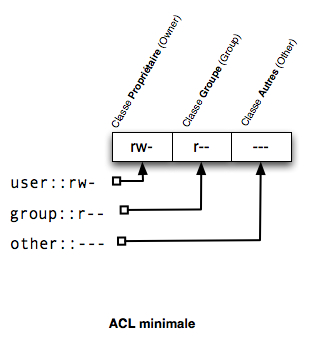
\includegraphics[height=3in]{img/acl-mapping-min.jpg}
\caption{ACL minimale}
\label{fig:img_acl-mapping1}
\end{figure}
 

\begin{figure}[htbp]
\centering
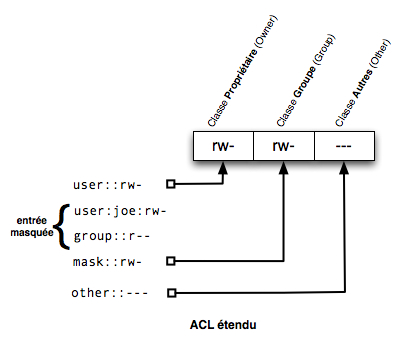
\includegraphics[height=3in]{img/acl-mapping-etendu.jpg}
\caption{ACL étendu}
\label{fig:img_acl-mapping2}
\end{figure}

 
Pour assurer le cohérence, quand une application change les permissions (par exemple le commande \emph{chmod}) les ACL sont modifiées de façon a reproduire cette modification.
 
On a dit que les permissions du masque sont calculées comme la limite supérieure de tous les entrées dans le classe groupe. Avec les ACLs étendus, on a besoin de masquer les permissions. Comme l'exemple du tableau (\ref{tab:masquee}), les permission des entrées de la classe groupe et qui aussi sont présentes dans le masque sont appliquées. Si une permission est absente dans le masque, c'est à dire qu'aucune entrée de groupe ne peut avoir cette permission, on dit dans ce cas que l'entrée est masquée.
 
\begin{center}
\begin{tabular}{|l|l|l|}
  \hline
    \multicolumn{3}{|c|}{La masque de permissionL} \\
  \hline
\textbf{Type} & \textbf{Format} & \textbf{Permission} \\
  \hline
Utilisateur nommée & user:jean:r-x & r-x\\
  \hline
Masque & mask::rw- & rw-\\
  \hline
\multicolumn{2}{|c|}{Permission Effective} & rw-\\
  \hline
\end{tabular}
\label{tab:masque}
\end{center}


Par être consistent, dans une application que utilise les ACL étendu, le permission du groupe propriétaire est toujours calculée comme la union entre le permission de ce groupe e la masque.  
 
\subsection{Algorithme de vérification}
 
Pour vérifier les droits d'accès d'une objet du système de fichier, il y a une algorithme assez simple.
 
%changer le titre et la langue
\begin{algorithm}
\caption{Vérifie se une utilisateur peut ou ne peut pas accéder une objet du système de fichier}
\label{algacl}
\begin{algorithmic}
\IF{l'identifiant de l'utilisateur du processus est le propriétaire}
\STATE l'entrée du propriétaire détermine l'accès
\ELSIF{l'identifiant d'utilisateur du processus correspond à une entrée d'utilisateur nommé dans la table des ACL}
\STATE l'entrée détermine l'accès
\ELSIF{un des identifiants de groupe du processus correspond au groupe propriétaire et l'entrée contient les permissions requises}
\STATE l'entrée détermine l'accès
\ELSIF{
un des identifiants de groupes correspond à un des groupe nommés et cette entrée contient les permissions requises}
\STATE l'entrée détermine l'accès
 
\ELSIF{
Un des identifiants de groupe du processus correspond au groupe propriétaire ou correspond à un des groupes nommés mais ni le groupe propriétaire ni aucun des groupes nommé contient les permission requises.}
\STATE ceci détermine que l'accès est interdit
 
\ELSE
\STATE l'entrée autre détermine l'accès
\ENDIF
 
%
\IF{
l'entrée qui détermine l'accès est l'entre du propriétaire ou l'entrée autres qui contient les permissions requises}
\STATE 
l'accès est autorisé
\ELSIF{l'entrée correspondante est l'utilisateur nom, ou le groupe propriétaire ou le groupe nommé et cette entrée contient les permissions requises et l'entrée masque contient aussi les permission. (ou il n'y a pas d'entrée masque)
}
\STATE l'accès est autorisé
 
\ELSE
\STATE l'accès n'est pas autorisé
\ENDIF
\end{algorithmic}
\end{algorithm}

 
\subsection{Héritage mécanisme}
\label{sec:heritage}
 
Le système POSIX règle non seulement les droits d'accès aux objets du système de fichiers, mais aussi le mécanisme d'Héritage. Les ACL sont partagés en deux types, les 
ACL d'accès (qu'on a vu jusqu'à maintenant) et les ACL par défaut qui comprennent les règles d'héritage.
 
Quand on parle de l'héritage, on parle des droits qui sont attribués aux objets du systèmes de fichiers au moment où ils sont crées. Il y a un seul type d'objet qui peut être associe avec les ACL par défaut les répertoires. Il faut dire que il n'y a pas de sens pour les ACL par défaut pour les fichiers car on ne peut pas créer un fichier à l'intérieur d'un fichier. Aussi les ACL par défaut et les 
ACL d'accès sont complètement indépendant.
 
Si un répertoire est crée dans une autre, si le première répertoire a ACL par défaut, avec le mécanisme d'héritage, le deuxième aura le même ACL que le premier (défaut  et accès). Les objets qui ne sont pas des répertoires, devons hériter les ACL par défaut seulement.
 
Chaque \emph{system call} qui crée les objets du système de fichier a un \emph{mode parameter}. Ce paramètre peut contenir neuf octets de permission pour chaque classe (propriétaire, groupe et les autres). Les permissions de chaque objet créée sont l'intersection des permissions définies pour les ACL par défaut et le \emph{mode parameter}.
 
Le système traditionnel a une commande pour désigner les modes de permissions par défaut pour les nouveaux fichiers et répertoires: le commande \emph{umask}. Quand il n'y a aucune ACL par défaut, la permission effective est déterminé par le \emph{mode parameter} moins les permissions configurés avec \emph{umask}.

\section{Problèmes arrivant les ACL POSIX}

\subsection{Compatibilité}

Il y deux situations qui problèmes qui être considérés quand on désire ajouter de nouvelles fonctionnalitées aux systèmes de fichiers (et donc au noyau): la mise à jour et comment un système qui n'a pas été mis à jour répond.
Aussi il faut s'il on a besoin d'un noyau plus léger, par exemple pour démarré le système de récupération, pouvoir désactiver les EAs. 

Quand on ajoute le support des ACL, tous les systèmes de fichiers qui n'on pas les ACL activées on a mécanisme de mise en place de leur support au moment du montage ou de manière automatique dans le première utilisation des EAs. 

On désire que les anciennes versions du noyau continent à marcher bien qu'il possède un système de fichier comportant des ACL. Dans un noyau où les ACL ne sont pas supportées, les systèmes de fichiers que implementent les ACL dans les répertoire, comme le ReiserFS, soient visibles. Il faut quand même que les droits de permission de ces répertoires soient configurés de façon à ce que les utilisateurs ne peuvent pas changer les informations de ces répertoire (ce qui mettrait en péril le système d'ACL). Avec le système de fichier ext2 et ext3, si on efface les fichiers avec contenant des ACL avec un noyau qui ne supporte les ACL, les ACL ne seront pas effacés, alors, on doit exécuter manuellement la vérification du système de fichiers pour le mettre à jour. 
 	
Aussi le mécanisme d'héritage pour un noyau ne supportant pas les ACL ne marchera pas. 

\subsection{Copie de Sécurité}

Un aspect très important et habituellement oublié est la copie de sécurité. Les outils comme \emph{cpio} et \emph{tar} ne connaissent pas les ACL. Cela veut dire qu'on perdra les information des ACL, si on en fait ces opérations avec ces outils car on perdra les EAs.

Une format appelé \emph{pax (Portable Archive Interchange)} a été défini pour POSIX pour résoudre ce problème. L'outil \emph{pax} peut comprendre les formats de \emph{cpio} et \emph{tar} et aussi le nouveaux format \emph{pax}. Ce nouveau format possède les \emph{extended headers} qui peuvent décrire les EAs. L'outil \emph{tar} peut le lire par contre il va perdre les informations des ACL. 

On peut aussi utiliser \emph{getfacl} et \emph{setfacl} comme des outils pour faire des copie de droits d'accès, par contre, leur utilisation n'est pas pratique. Si on désire effectuer une copie de sécurité complète ces outils sont adéquat mais pas pour quelques fichiers. 

\section{Implèmentassions des ACL POSIX}
 
%il faut ajouter references
Les ACLs sont fréquemment implémentées comme des extensions du noyau, c'est à dire des modules un système LINUX. L'objectif de cette section est d'expliquer de manière globale l'implémentions des ACL. 
 
"Les ACLs sont des informations de taille variable qui sont associées avec les objets du systéme de fichier"\cite{aclsuse}. Plusieurs implémentations des ACLs sont possibles. Par exemple, avec Solaris, dans le système de fichier UFS\cite{acl_permission} chaque \emph{inode} peut avoir une ACL. S'l en a une, il doit avoir l'information \emph{i\_shadow}, un pointeur pour un \emph{shadow inode}. Les \emph{shadow inode} sont comment fichiers réguliers d'utilisateurs. Différent fichiers avec les mêmes ACL peut avoir pointeurs pour le même \emph{shadow inodes}. Les information des ACL sont garde dans les bloc de données de chaque \emph{shadow inodes}.
 
La capacité d'associer des informations avec des fichiers est utilise dans plusieurs fonctions du système de exploitation. De ce fait, la plupart des systèmes \emph{UNIX-like} (de type Linux) on trouve les Attributs étendus (\emph{Extended Attributes (EAs)}). Les ACL sont implémentées avec ce mécanisme.


La manpage \cite{aclsuse} \emph{attr(5)} contient des explications précises sur les EAs dans Linux. Comme les variables des processus, les EAs sont des paires (nom, valeur) associées de manière persistantes avec les objets du système de fichiers. Les appels système Linux pour les ACL, sont employées pour opérer sur les informations contenues dans ces paires dans le espace d'adresse du noyaux. Aussi l'implémentation des EA et des appels système dans FreeBSD sont documentés par l'article de Robert Watson\cite{trust}. Cette article content aussi une comparaison de plusieurs implèmentations de ces système.
 
Dans le monde linux, ajouter le support aux ACL en les implémentant avec des EA limitée offre plusieurs avantages: un grande facilité d'implémentation, les opération sont atomiques et l'interface est sans état donc il n'y a aucune surcharge au niveau \emph{file handlers}. On ne doit pas oublier que l'implémentation doit être efficace car les ACL souvent utilisées.
 
\subsection{Les EAs et les systémes de fichiers}
 
Chaque système de fichier a une différent implémentation pour les EAs. On peut penser qu'une solution partagée pour l'ensemble des systèmes pourrait être plus efficace. Par exemple, si on prend une solution simple où chaque objet du système de fichiers a les EAs, un répertoire avec un fichier qui a le clés EA comment le nom et le contenu comment le valeur. Cette implémentation consommerait beaucoup de espace, étant donne que les blocks du système de fichier seront gaspilles pour conserver petit morceaux de donne, aussi ce solution perdrait les temps pour chercher ces information a chaque accès de fichier. Aux frais de ces problèmes chaque système tire profit de ces qualités pour ajouter le supporte aux EAs.
 
\subsubsection{Ext (2,3 et 4)}
 
Les ACL dans Ext suivent le principe linux: "La solution la plus simple qui marche" et pour cette raison subviennent quelques limitations. D'autres solutions existent, par contre, elle sont difficiles à ajouter au noyau de manière satisfaisante\cite{ext_acl}.
 
La solution actuelle ajoute aux \emph{i\_node} une entrée qui s'appelle \emph{i\_file\_acl}. Cette entrée, si différent de 0, est une ponter sur un bloc d'EAs. Ce bloc d'EAs a les informations de nom et valeur de tous les ACL du fichier indique pour cet \emph{i\_node}.
 
Le mécanisme a aussi une optimisation. Deux fichiers avec le même ensemble de ACL point vers le même bloc d'EAs. Le système garde une \emph{hash map} avec les \emph{checksum} des blocs d'EAs et leurs adresse. Chaque block a aussi un compteur de référence, comme les liens \emph{hard}. Ce mécanisme détermine aussi que ce compteur là ne peut pas avoir plus que 1024 références. Il s'agit d'une mesure de sécurité en cas de perte des données.
 
Aussi une limitation est imposée: toutes les données des EAs d'un fichier doivent occuper un bloc d'EAs ayant une taille de 1, 2 ou 4 KBs.
 
 
\subsubsection{JFS}
 
Dans JFS, les EAs sont ajoutées dans une liste consécutive de blocs contigus (un entent).  Cela veut dire que chaque paire (nom,valeur) est gardée en séquence et que chaque valeur de la paire ne peut pas être plus grande que 64kb. Si les EAs sont assez petites, elles pourrons être gardées dans le même lieu que les informations du fichier. De ce façon, il n'y a pas les limitations d'ext3.
 
\subsubsection{XFS}
XFS est le système de fichiers le plus simple pour implémenter les EA. Les paires d'EA de petite tailles sont stockées directement dans l'inode, celles de taille moyenne sont stockées dans les blocs feuilles de l'arbre binaire et pour celle de grande taille, dans un arbre binaire complet.

XFS peut configurer la taille de sa table d'inodes. La taille minimale est de 256 octet et la taille maximale peut aller jusqu'à la moitié des blocs du système de fichier. Dans le cas où on a une table de taille minimale, celle-ci n'est pas assez grande pour accueillir les ACLs. On doit alors les stocker de manière externe dans l'arbre binaire. Si on augmente la taille de la table les ACL pourront y être stockées. Les ACL étant très souvent interrogées par le système, cela augmente les performances en terme de temps d'accès au détriment de l'espace disque qu'elles consomment.
XFS n'a pas de mécanisme de partage des attributs. La taille individuelle des attributs est limitée à 64Kb.
 
\subsubsection{ReiserFS}

ReiserFS support le \emph{tail merging} qui permet à plusieurs fichiers de partager le même bloc pour stocker leurs données. Cela rend le système très efficace pour s'il on possède de nombreux fichiers de petite taille. De l'autre côte cette technique consomme beaucoup de ressources CPU. 
	
Comme le ReiserFs peut facilement manipuler des petits fichiers, les EA peuvent être implémentées sous forme de petits fichiers. Pour chaque fichiers qui a un EA, un dossier spécial (qui est souvent cache) est créé avec un nom dérive de son inode. Dans ce dossier chaque EA est stockée dans un fichier sépare qui a pour nom le nom de l'attribut. Le contenu de chaque fichier est la valeur de l'attribut.

Le système ReiserFS n'implémente pas le partage d'attributs mais la création d'une extension pour le gérer est possible. La taille individuelle des attributs est limitée à 64Kb.

\section{Système de fichiers à distance}
%VOIR
Dans le contexte des système de fichier à distance nouveaux complication arrive. Ce système sont usuellement une couche permettent  une système de fichier être partage dans une réseaux. Si les décision d'accès sont tous laisse au serveur, une problème de performance arrive, par contre, se quelques de ces information sont délègue aux cliente, parfois la sécurité est compromise. Il y a aussi le problème de comptabilité, quand différentes systèmes d'exploitation implementent le même protocole de système de fichier à distance. On va voir ces deux problème, une avec le NFS (Network File System) et autre avec CIFS (Common Internet File System). 

\subsection{NFS}
%VOIR
Pour ajouter le support ACL au système NFS: une extension au protocole NFS permettent la manipulation des ACL à distance et une modification du algorithme de vérification de droits.

Dans la deuxième version du protocole NFS, une partie de la décision de qui a le droit d'accéder aux fichier se déroule dans le cliente. Pour une question de performance il y a une cache de fichier dans la côte cliente. L'algorithme que prend ces choix suppose que les ID (d'utilisateur et groupe) et les octets de permission sont suffisant. Ce supposition est évidement incorrect quand on a les ACL. Cette choix c'est aussi la raison de plusieurs problème de sécurité dans NFS, lorsque une ordinateur est capable de accéder le système à distance cas on a le pouvoir de \emph{root} dans cette machine, on peut tromper l'algorithme NFS a nous donner les information des autres utilisateurs donne que on peut changer notre valeur d'ID a volonté.

On peut penser que la solution de ce problème doit venir du choix de une nouvelle façon de choix qui reste dans la côte cliente. Par contre, cela ne marcherais pas quand les différents serveurs implementent différents modèle de permissions. 

Comme solution, le NFSv3 implement le appel RCP \emph{ACCES}, par contre, cette appel est trop lourd et pose les problème de performance même pour les système qui n'ont pas ACL, alors, dans le version trois on a le pouvoir de spécifier l'option \emph{noacl} pour désactiver le support a cette appel. 

Le NFSv4 finalement résoudre le problème avec ces propre ACL, par contre, ces ACL ne sont pas compatible avec les POSIX ACL. Ces ACL sont disponible gratuitement pour l'entreprise Sun, depuis le trois mars de 2003 sur le site http://acl.bestbits.at/. 

\subsection{Samba}
%VOIR
Le système de fichier \emph{NT File System} (NTFS) support les ACL d'une façon très particulière. Le protocole CIFS\cite{cifs}, utilisée pour partager les imprimants e les fichier dans une réseaux aussi supporte les ACL ajouter au NTFS. Une implementation livre (\emph{Open Source}) du CIFS s'appelle Samba et offre les service de cliente et aussi de partage de imprimants e fichiers Linux pour les utilisateurs Windows. Samba aussi permettre les ACL POSIX d'être modifier dans une système \emph{Windows}.  

Le modelé des ACL windows diffère beaucoup de les ACL POSIX de une façon que on trouve impossible une intégration complète. Voici une liste de les principales différences entre les deux ACL:

\begin{itemize}
	\item Les ACL windows supportant a peu prés dix différentes permissions pour chaque entré dans une ACL. Entre eux, on trouve \emph{append}, \emph{delete}, \emph{change permission},\emph{take ownership} et \emph{change ownership}.
	\item Dans les ACL POSIX l'accès est défini pour une algorithme que cherche le \emph{matching} plus proche entre les ACL disponible. Dans le monde \emph{Windows} le permission sont cumulative, par contre, on peu les restreigne avec les entré \emph{DENY ACL}.
	\item Il n'y a pas les entrée \emph{DENY} dans les ACL POSIX. L'unique façon de restreigne l'aces c'est pour le \emph{matching}.
	\item Le mécanisme d'héritage dans \emph{Windows} permettre que une modification de les ACL se propage dans l'hiérarchie dessous le répertoire.
	\item Il n'y a pas l'entrée masque dans les ACL \emph{Windows}.
\end{itemize}

\section{ACL POSIX en use}

Dans cette session on verrais les uses des ACL dans les système d'aujourd'hui. 

\subsection{ACL Kernel Patches}
Les ACL \emph{patchs} ont été ajouté dans les noyaux Linux depuis Novembre 2002. Ces \emph{patchs} implémentent le POSIX 1003.1e draft 17 et elles ont été ajoutées dans la version 2.5.46 du noyau. Donc le support des ACL et aussi présent dans le dernière version du noyau actuel. Depuis 2004 le support aux ACL est disponible pour les système de fichiers Ext2, Ext3, IBM JFS, ReiserFS et SGI XFS. Les ACL sont supportés aussi pour le système NFS, par contre, quelques problèmes de sécurité sont connus\cite{nfs_problem}. 

Aujourd'hui il est assez simple d'ajouter le support aux ACL dans les distributions Linux comme Ubuntu ou Debian. On verra marche à suivre pour ajouter ce support après.

\subsection{Mac OSX}
Le système de exploitation Mac OSX (10.6.2 Snow Leopard au moment où ces lignes sont écrites) supporte aussi les ACL et elles sont complètement intégrées à l'interface de l'utilisateur (\ref{fig:img_mac-acl}). 

\begin{figure}[htbp]
	\centering
		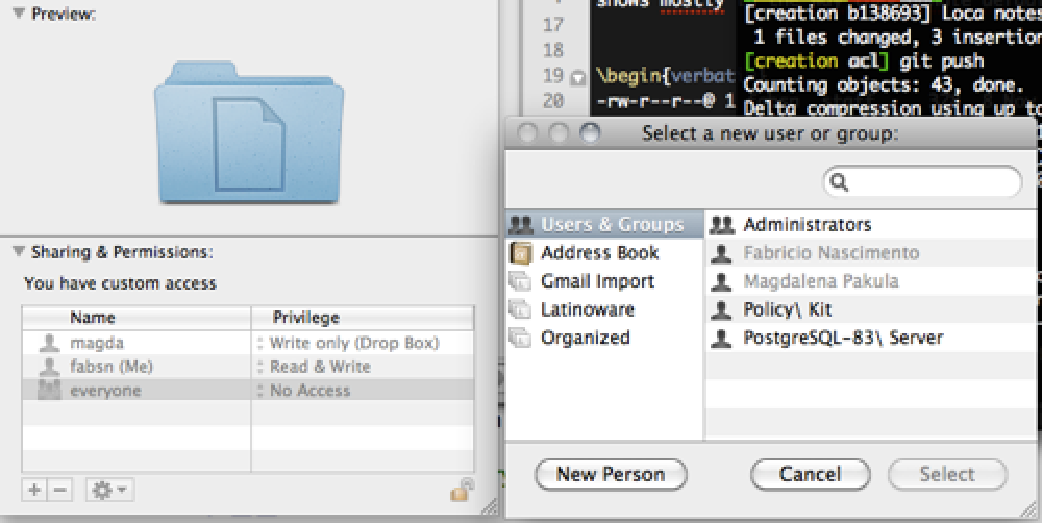
\includegraphics[height=2in]{img/mac-acl.pdf}
	\caption{Mac OSX Snow Leopard ACL Interface}
	\label{fig:img_mac-acl}
\end{figure}

\subsection{ACL dans Linux}


%References 
Les dernières versions des distributions de Debian ou Ubuntu, comme Ubuntu 9.10, viennent avec le support des ACL. Dans Ubuntu 8.10 l'application Nautilus, qui est responsable pour la visualisation du système de fichiers, contenait une interface pour les ACL, qui a apparemment disparues dans les version suivantes et Nautilus dans Ubuntu 9.10 ne l'intègre pas. La marche à suivre pour ajouter le support des ACL dans le Ubuntu 9.10 est la suivante:

\begin{verbatim}
1) Installer le paquet des acl. 
user@ubuntu:$ sudo apt-get install acl

2) Ajouter l'option 'acl' au système de fichier
 correct dans le /etc/fstab, comme:
UUID='gros sequence' /dev/hda6 /home ext3 rw,auto,acl 0 1

3) Remonter le système de fichiers avec la nouvelle option
user@ubuntu:$ sudo mount /home -o remount

\end{verbatim}

\section{Exemples d'utilisation}
\subsection{Ajouter les ACL aux fichiers}

On peut utiliser le commande 'ls -la' pour regarde les permissions. Si un fichier contient information de sécurité avancée (comme les ACL) on va voir le caractère '+', comme dans la sortie du command 'ls' ci-dessous (\ref{verb:ls}). Un fichier avec devant une '@' veut dire que le fichier contient EAs. 

\begin{center}
\label{verb:ls}
\begin{verbatim}
-rw-r--r--@ 1 fabsn  staff     378  8 Nov 15:29 Makefile
-rw-r--r--@ 1 fabsn  staff     618  8 Nov 15:59 README
-rw-r--r--@ 1 fabsn  staff      31  8 Nov 15:15 draft-header
-rw-r--r--@ 1 fabsn  staff      24  8 Nov 15:15 header
drwxr-xr-x@ 2 fabsn  staff     102  8 Nov 15:26 img
-rw-r--r--  1 fabsn  staff     972  8 Nov 15:57 rapport-draft.aux
-rw-r--r--  1 fabsn  staff   18129  8 Nov 15:57 rapport-draft.log
drwxrwxr-x+ 3 fabsn  staff	  1024  8 Nov 20:23 repertoire
\end{verbatim}
\end{center}

Pour voir les ACL on doit utiliser la commande \emph{getfacl}. Les informations sont ajoutées en accord avec les définitions données dans l'introduction sur les ACL dans la tableau \ref{tab:entree}. 

\begin{verbatim}
fabsn@vadmin:/media/esisar$ getfacl repertoire/
# file: repertoire/
# owner: root
# group: root
user::r-x
user:daemon:rwx
user:bin:rwx
user:fabsn:rwx
user:nobody:rwx
group::r-x
group:admin:rwx
group:fabsn:rwx
mask::rwx
other::r-x	
\end{verbatim}

Aussi il y a la commande \emph{setfacl} pour modifier, ou ajouter des permissions ACL. La commande ci-dessous modifie (-m) par exemple les permissions du l'utilisateur \emph{fabsn} pour le répertoire. 

\begin{verbatim}
setfacl -m user:fabsn:r-x repertoire
\end{verbatim}


\subsection{Exemple ACL d'accès}

Voici un exemple d'utilisation que l'on peut trouver dans l'article d'Andreas Gruembacher\cite{aclsuse}.

On part de la création d'un répertoire avec l'application de umask de valeur 027 (octal). Cela veut dire qu'il va désactiver le droit d'écriture pour le groupe propriétaire et l'écriture, la lecture et l'exécution pour les autres.

\begin{verbatim}
$ umask 027 
$ mkdir dir 
$ ls -dl repertoire
	drwxr-x--- ... user group ... repertoire
\end{verbatim}

La lettre "d" montre que l'objet "répertoire" est un répertoire suivi par les octets de permission "rwxr-x---". Les "..." dans la sortie masquent les informations inutiles pour cet exemple. Ces permissions basiques ont toujours une représentation dans les ACL, pour les afficher on fait:

\begin{verbatim}
$ getfacl repertoire
# file: repertoire 
# owner: user 
# group: goup
user::rwx
group::r-x
other::---
\end{verbatim}

Le trois premières lignes après commande (qui démarrent par le \#) nous donnent les informations sur les propriétaires (groupe et utilisateur) et le nom du fichier. Après chaque ligne vient la liste des ACL. Cet exemple montre un ACL minimal. Si par exemple on ajoute les permissions "rwx" pour l'utilisateur "jean" avec la commande \emph{setfacl} on va avoir des ACL étendus.

\begin{verbatim}
$ setfacl -m user:jean:rwx repertoire
$ getfacl --omit-header repertoire 
	user::rwx 
	user:jean:rwx	
	group::r-x 
	mask::rwx 
	other::---
\end{verbatim}

Il faut rappeler que le commande \emph{setfacl} a été employée avec l'argument \emph{-m (modify)}. Pour observer les résultats on utilise encore une autre fois \emph{getfacl}. Il faut savoir que l'argument \emph{--omit-header} cache les premières 3 lignes avec les informations sur les propriétaires.  

Tout d'abord on peut voir que l'entrée masque a été ajoutée. Ces permissions sont créées comme l'union entre les permissions de jean et du groupe propriétaire. Le masque doit être une valeur qui ne masque aucune permission.  

\begin{verbatim}
ls -dl repertoire
	drwxrwx---+ ... user group ... repertoire
\end{verbatim}

Si on se rappelle le dernier exemple, le groupe propriétaire n'a pas le droit en écriture (\emph{group::r-x}), par contre, la classe groupe a ce droit. C'est pour cela que quand on calcule effectivement le droit avec la permission de jean, le masque devient "rwx".

Le prochain exemple montre comment les ACL sont modifiés avec l'emploi de commande \emph{chmod}. On va effacer la permission d'écriture de la classe groupe.

\begin{verbatim}
$ chmod g-w repertoire 
$ ls -dl repertoire 
	drwxr-x---+ ... user group ... repertoire 
$ getfacl --omit-header repertoire 
user::rwx 
user:jean:rwx 	#effective:r-x
group::r-x 	
mask::r-x 
other::---

\end{verbatim}

Si une ACL entrée contient une permission désactivé pour le masque, \emph{getfacl} ajoute un commentaire qui montre cette différence.

On va voir maintenant ce qui se passe quand on rajoute la permission. 

\begin{verbatim}
$ chmod g+w repertoire 
$ ls -dl repertoire 
	drwxrwx---+ ... user group ... repertoire 
$ getfacl --omit-header repertoir 
user::rwx 
user:jean:rwx 
group::r-x
mask::rwx
other::---
\end{verbatim}

Cet exemple montre que les changements effectués avec la commande \emph{chmod} ne détruises pas les ACL. Les opérations sont complètement réversibles et les permissions d'avant et d'après les deux opérations sont les mêmes: c'est une caractéristique très importante des ACL POSIX. 

\subsection{Exemple des ACL par défaut}

Avec l'argument -d, on peut afficher les ACL par défaut d'un répertoire. 

\begin{verbatim}
$ setfacl -d -m group:admin:rwx repertoire 
$ getfacl --omit-header repertoire 
user::rwx
user:jean:rwx
group::rwx 
mask::rwx
other::---
default:user::rwx
default:group::r-x
default:group:admin:rwx
default:mask::r-x
default:other::---
\end{verbatim} 

Les ACL par défaut viennent après les ACL d'accès et sont préfixés par la chaîne de caractères "default::". D'habitude quand on ajoute une nouvelle règle dans les ACL d'accès comme on a fait pour le groupe \emph{admin} n'affecte pas les ACL par défaut. Par contre, il y a une extension sur Linux qui ajoute de manière automatique la règle dans les ACL par défaut. 

Il faut voir qu'il n'y a aucune entrée pour jean dans les défaut ACL, alors, jean n'aura pas accès dans le nouvelle objet crée dans le répertoire (sauf c'est membre d'un groupe qui a les permissions). 

En accord avec le mécanisme d'héritage que l'on vu dans le page \ref{sec:heritage}, le sous-répertoire doit hériter des ACL de son père. Par défaut, la commande \emph{mkdir} utilise un \emph{mode parameter} de 0777 pour cet appel de système. On observe:

\begin{verbatim}
$ mkdir repertoire/subrep 
$ getfacl --omit-header repertoire/subrep 
user::rwx 
group::r-x 
group:admin:r-x 
mask::r-x 
other::--- 
default:user::rwx 
default:group::r-x 
default:group:toolies:r-x 
default:mask::r-x 
default:other::---
\end{verbatim}

Pour les fichiers cela arrive aussi. La commande \emph{touch} utilise le \emph{mode parameter} 0666. Toutes les permissions qui ne sont pas présente dans le \emph{mode parameter} sont écrasées.

Enfin, aucune permission n'a été écrasée dans le groupe classe, cependant, la masque a été appliqué. Cette politique s'assure que par exemple les application comme les compilateurs peuvent fonctionner avec les ACL même s'ils ne supportent ce mécanisme. Ils peuvent créer des fichiers avec des permissions restreintes et ensuite donner les permissions d'exécution et sans que les groupes et autres permissions ne soient affectés.

\section{Conclusion}
%VOIR
C'est suivant dans une grande nombre d'aires dans l'informatique que l'addiction de quelque fonctions, même que parfois nécessaires, résoudre dans une augmentation de complexité et apportent quelques nouveaux problèmes. 

Les ACL POSIX dans le monde UNIX sont un exemple de ce comportement. Elles se traitent d'un implémentation solide et que peu interfère avec la performance des système, quand même, les système de fichier, comme NFS, soufrent des problèmes que vient avec ce supporte.

Dans la plupart des besoin associé au contrôle de permission pour les utilisateurs, le modèle traditionnel se fait suffisant, alors, il faudrait qu'on sache quand serais nécessaire l'utilisation de ce modelé étendu. 

\newpage

\begin{thebibliography}{9}
 
\bibitem{aclsuse}
  Andreas Gruenbacher,
  \emph{POSIX Acess Control Lists on Linux}.
  http://www.suse.de/~agruen/acl/linux-acls/online/,
  2003.

\bibitem{ieee1}
    IEEE Std 1003.1-2001 (Open Group Technical Standard, Issue 6), 
	Standard for Information Technology--Portable Operating System Interface (POSIX) 2001. 
	ISBN 0-7381-3010-9. 
	http://www.ieee.org/

\bibitem{ieee2}
    IEEE 1003.1e and 1003.2c: Draft Standard for Information Technology--Portable Operating System Interface (POSIX)--Part 1: System Application Program Interface (API) and Part 2: Shell and Utilities, draft 17 (withdrawn). 
	October 1997. 
	http://wt.xpilot.org/publications/posix.1e/

\bibitem{ftp}
	Mark Lowes: 
	Proftpd: 
	A User's Guide March 31, 2003. 
	http://proftpd.linux.co.uk/

\bibitem{posix17}
    Winfried Trümper: Summary about Posix.1e. Publicly available copies of POSIX 1003.1e/1003.2c. February 28, 1999. "http://wt.xpilot.org/publications/posix.1e/"

\bibitem{acl_permission}
	Jim Mauro: Controlling permissions with ACLs. Describes internals of UFS's shadow inode concept. SunWorld Online, June 1998.

\bibitem{trust}
	Robert N. M. Watson: Introducing Supporting Infrastructure for Trusted Operating System Support in FreeBSD. BSDCon 2000, Monterey, CA, September 8, 2000. http://www.trustedbsd.org/docs.html
	
\bibitem{nfs_problem}
	Andreas Grünbacher: Linux Extended Attributes and ACLs. Session "Known Problems and Bugs". http://acl.bestbits.at/problems.html
	
\bibitem{ext_acl}
	Andreas Dilger: [RFC] new design for EA on- disk format. Mailing list communication, July 10, 2002. http://acl.bestbits.at/pipermail/acl-devel/2002-July/001077.html
	
\bibitem{ext_jfs}
	Austin Common Standards Revision Group. http://www.opengroup.org/austin/

\bibitem{cifs}
	Storage Networking Industry Association: Com- mon Internet File System Technical Reference. Technical Proposal, March 2002. http://www.snia. org/tech activities/CIFS/

\end{thebibliography}


\end{document}


